\section{Décomposition en activités des processus du PIC}

Le Système de Management de la Qualité défini par le PIC \nomPIC{} se décompose en trois processus~:
\begin{itemize}
 \item Manager la qualité : assurer, suivre et améliorer la qualité udu pic ; 
 \item Conduire le projet ;
 \item Réaliser les produits. \\
\end{itemize}

Un pilote (membre de PIC) est attribué à chaque processus. Sa mission sera de s'assurer du bon fonctionnement du processus et de gérer les risques liés à ce dernier.

Pour diviser le projet en processus, nous avons utilisé un Work Breakdown Structure(WBS). Le WBS est visible sur la figure \ref{WBS1}.

\begin{figure}[H]
\centering
 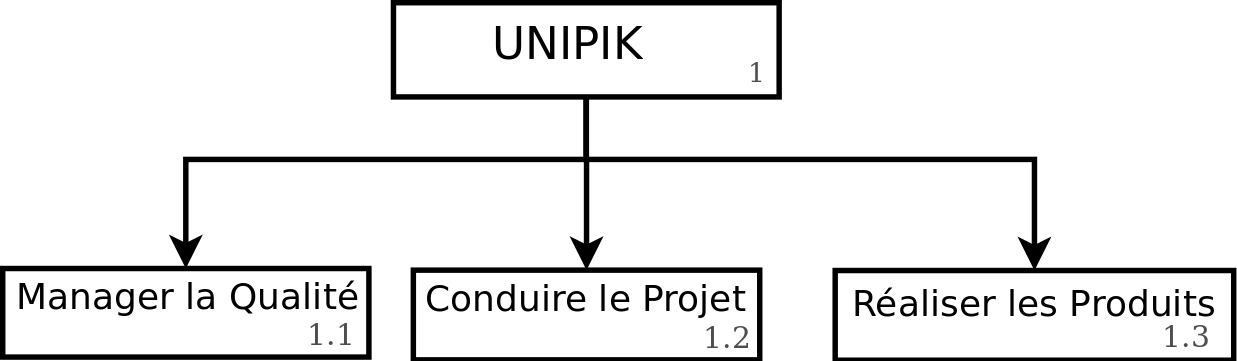
\includegraphics[width=14cm]{images/organigrammeProcessusPic.png}
 \caption{Processus du PIC~: projet \nomEquipe{}}
 \label{WBS1}
\end{figure}

 Dans le cas ou il y a des évolutions, les modifications seront présentées dans la prochaine mise à jour.
\newpage
 
\section{Processus : Manager la Qualité}
\label{ProcessusQualite}
Ce processus se décompose en trois parties~:
\begin{itemize}
\item La mise en place de la Qualité au sein du PIC (rédaction du PQ et organisation de l'équipe PIC) ; 
\item Le suivi de la Qualité tout au long du projet ; 
\item L'amélioration de la Qualité tout au long du PIC (définition d'objectifs et d'axes d'amélioration et mise à jour des documents). 
\end{itemize}
\subsection{\WBSCourt{}}
Le Système de Management de la Qualité au moment de la diffusion de ce document est présenté par une WBS, disponible en figure 3.2.
Le pilote de ce processus sera \Pierre{} en tant que \RQ{}.

\begin{figure}[H]
\centering
 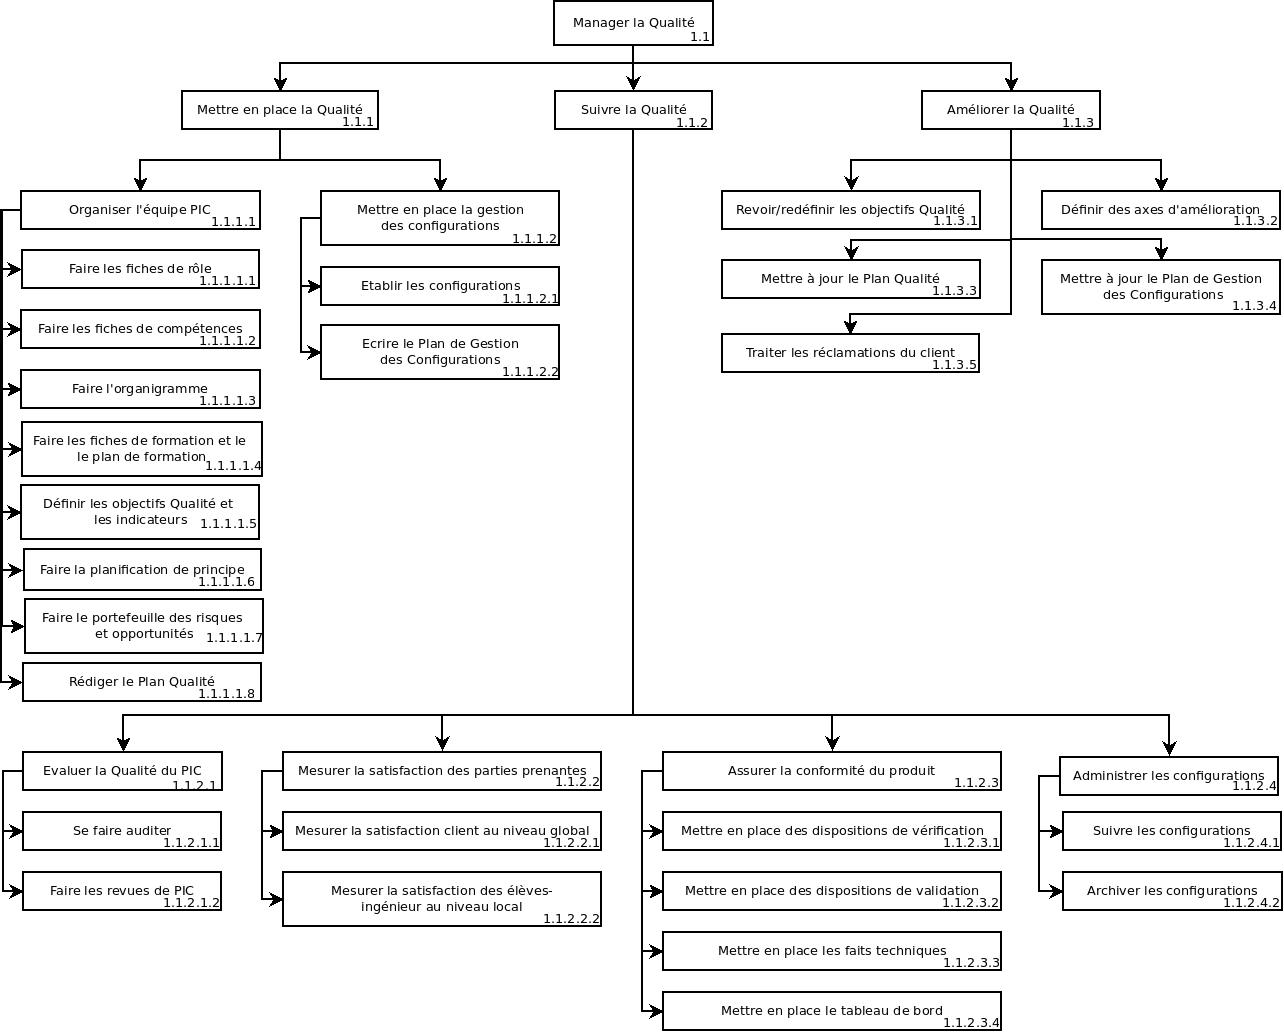
\includegraphics[width=19cm,angle=-90]{images/managerQualite.png}
 \caption{\WBSCourt{}~: Manager la Qualité}
 \label{WBS2}
\end{figure}

\newpage

\subsection{Références aux procédures}
\begin{landscape}
\begin{longtable}{|p{3.0cm}|p{14.5cm}|p{5cm}|}
	% En-tête du tableau
	\hline
	\rowcolor[gray]{0.65}\textbf{N° WBS} & \textbf{Intitulé du processus / de l'activité / de la tâche} & \textbf{Procédure en référence}\\
	\hline
	\endhead % (répétée, sinon \endfirsthead)

	% Corps du tableau


        \ligneMaj{1.1}{Manager la qualité}{Chapitre 4 - \DGQDEUXCourt{}}

        \ligneSup{1.1.1}{Mettre en place la qualité}{Partie 4.2 - \DGQDEUXCourt{}}
        \ligneMed{1.1.1.1}{Organiser l'équipe PIC}{Partie \ref{Organisation} - \PQCourt{}}
        \ligneSub{1.1.1.1.1}{Faire les fiches de rôle}{Partie 3.2.2 - \DGQDEUXCourt{}}
        \ligneSub{1.1.1.1.2}{Faire les fiches de compétences}{Partie \ref{CompetencesEtFormations} - \PQCourt{}}
        \ligneSub{1.1.1.1.3}{Faire l'organigramme}{Partie \ref{CompetencesEtFormations} - \PQCourt{}}
        \ligneSub{1.1.1.1.4}{Faire les fiches de formation et le plan de formation}{Partie \ref{CompetencesEtFormations} - \PQCourt{}}
        \ligneSub{1.1.1.1.5}{Définir les objectifs Qualité et les indicateurs}{Partie \ref{Organisation} - \PQCourt{}}
        \ligneSub{1.1.1.1.6}{Faire la planification de principe}{Partie \ref{CompetencesEtFormations} - \PQCourt{}}
        \ligneSub{1.1.1.1.7}{Faire le portefeuille des risques et opportunités}{Partie \ref{CompetencesEtFormations} - \PQCourt{}}
        \ligneSub{1.1.1.1.8}{Rédiger le Plan Qualité}{Partie 4.2.2 - \DGQDEUXCourt{}}
        \ligneMed{1.1.1.2}{Mettre en place la gestion des configurations}{Partie 7.2 - \DGQDEUXCourt{}}

        \ligneSup{1.1.2}{Suivre la Qualité}{Partie 4.3 - \DGQDEUXCourt{}}
        \ligneMed{1.1.2.1}{Evaluer la Qualité du PIC}{}
        \ligneSub{1.1.2.1.1}{Se faire auditer}{Partie 4.3.4 - \DGQDEUXCourt{}}
        \ligneSub{1.1.2.1.2}{Faire les revues de PIC}{Partie 4.3.3 \DGQDEUXCourt{}}
        \ligneMed{1.1.2.2}{Mesurer la satisfaction des parties prenantes}{Partie 4.3.1 \DGQDEUXCourt{}}
        \ligneSub{1.1.2.2.1}{Mesurer la satisfaction client au niveau global}{Partie 3.1.1 - \DGQTROISCourt{}}
        \ligneSub{1.1.2.2.2}{Mesurer la satisfaction des élèves-ingénieur au niveau local}{Partie 3.1 - \DGQTROISCourt{}}
        \ligneMed{1.1.2.3}{Assurer la conformité du produit}{}
        \ligneSub{1.1.2.3.1}{Mettre en place des dispositions de vérification}{Partie 4.3.2 - \DGQDEUXCourt{}}
        \ligneSub{1.1.2.3.2}{Mettre en place des dispositions de validation}{Partie 4.3.2 - \DGQDEUXCourt{}}
        \ligneSub{1.1.2.3.3}{Mettre en place les faits techniques}{Partie 4.3.5 - \DGQDEUXCourt{}}
        \ligneSub{1.1.2.3.4}{Mettre en place le tableau de bord}{Partie 4.3.6 - \DGQDEUXCourt{}}
        \ligneMed{1.1.2.4}{Administrer les configurations}{Partie 7.3 - \DGQDEUXCourt{}}
        \ligneSub{1.1.2.4.1}{Suivre les configurations}{Partie 8 - \pgcCourt{}}
        \ligneSub{1.1.2.4.2}{Archiver les configurations}{Partie 8 - \pgcCourt{}}

        \ligneSup{1.1.3}{Améliorer la Qualité}{Partie 4.4 - \DGQDEUXCourt{}}
        \ligneMed{1.1.3.1}{Revoir/redéfinir les objectifs Qualité}{Partie 5.2.1 - \DGQTROISCourt{}}
        \ligneMed{1.1.3.2}{Définir des axes d’amélioration}{Partie 4.4.2 - \DGQDEUXCourt{}}
        \ligneMed{1.1.3.3}{Mettre à jour le Plan Qualité}{Partie 4.4.3 - \DGQDEUXCourt{}}
        \ligneMed{1.1.3.4}{Mettre à jour le Plan de Gestion des Configurations}{Partie 4.4.3 - \DGQDEUXCourt{}}
\end{longtable}
\end{landscape}

\newpage



\section{Processus : Conduire le PIC}
\subsection{\WBSCourt{}}
\label{ProcessusConduirePic}
Une WBS qui explique la Conduction du Projet au moment de la diffusion de ce document est disponible en figure 3.3.
Le pilote de ce processus sera \Sergi{} en tant que \CP{}.

\begin{figure}[H]
\centering
 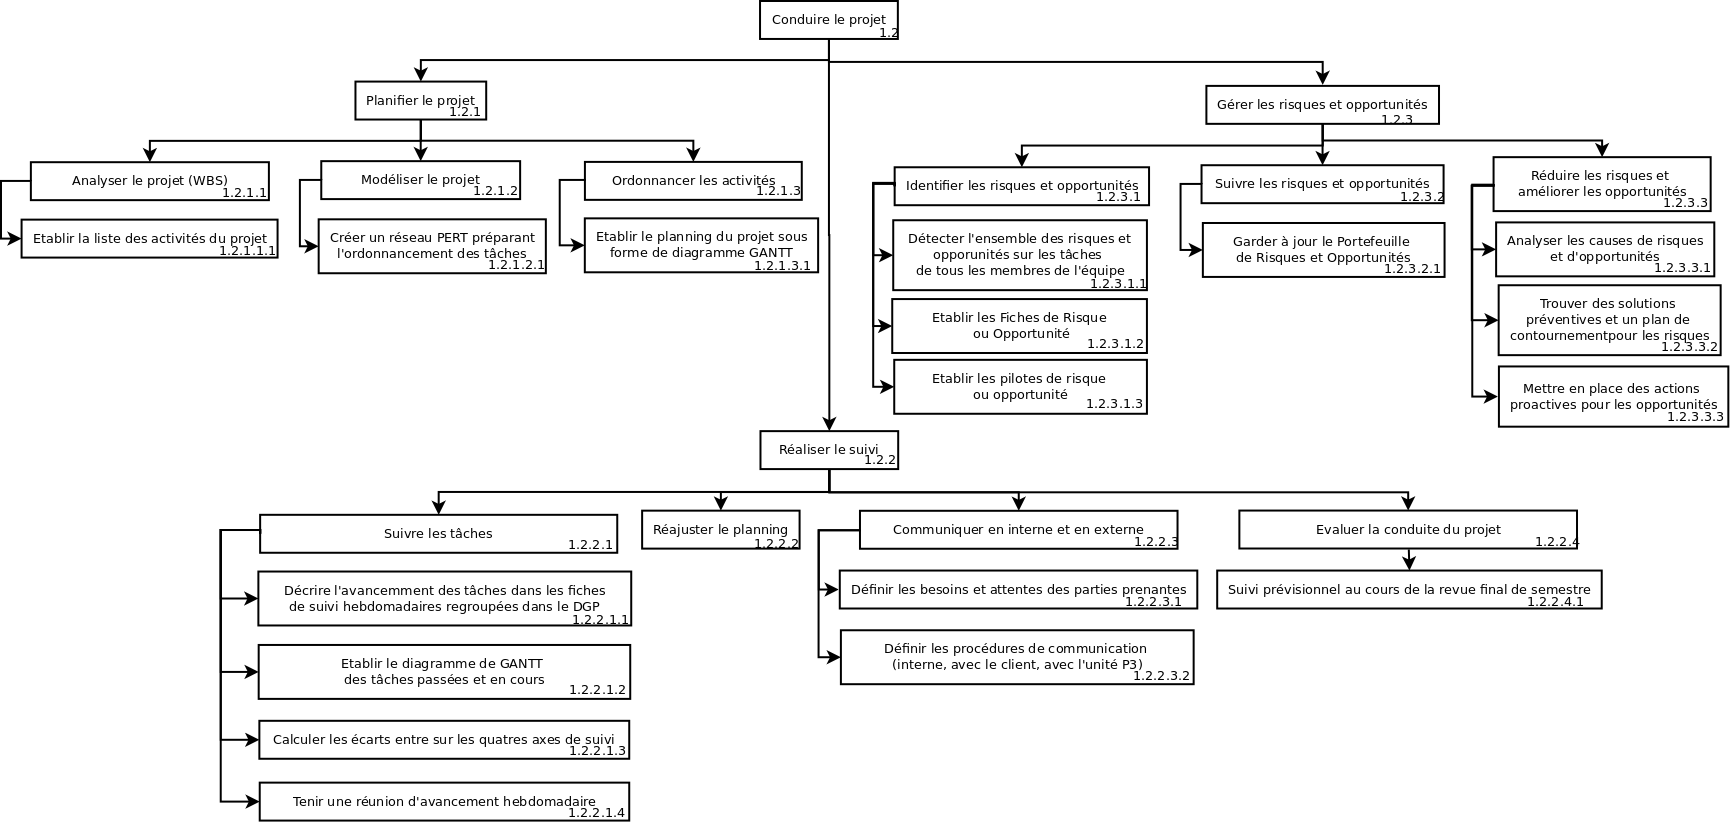
\includegraphics[width=24cm,angle=-90]{images/ConduireLeProjet.pdf}
 \caption{\WBSCourt{}~: Conduire le PIC}
 \label{WBS3}
\end{figure}


\newpage
\begin{landscape}
\subsection{Références aux procédures}
		\small
		\begin{longtable}{|p{3.0cm}|p{14.5cm}|p{5cm}|}
			% En-tête du tableau
			\hline
			\rowcolor[gray]{0.65}\textbf{N° WBS} & \textbf{Intitulé du processus / de l'activité / de la tâche} & \textbf{Procédure en référence}\\
			\hline
			\endhead % (répétée, sinon \endfirsthead)

			\ligneMaj{1.2}{Conduire le projet}{Chapitre 5 - \DGQDEUXCourt{}}

			\ligneSup{1.2.1}{Planifier le projet}{Partie 5.2 - \DGQDEUXCourt{}}
			\ligneMed{1.2.1.1}{Analyser le projet (WBS)}{Partie 5.2.1 - \DGQDEUXCourt{}}
			\ligneSub{1.2.1.1.1}{Établir la liste des activités du projet}{}
			\ligneMed{1.2.1.2}{Modéliser le projet}{Partie 5.2.2 - \DGQDEUXCourt{}}
			\ligneSub{1.2.1.2.1}{Créer un réseau PERT préparant l'ordonnancement des tâches}{}
			\ligneMed{1.2.1.3}{Ordonnancer les activités}{Partie 5.2.3 - \DGQDEUXCourt{}}
			\ligneSub{1.2.1.3.1}{Établir le planning du projet sous forme de diagramme GANTT}{}


			\ligneSup{1.2.2}{Réaliser le suivi}{Partie 5.3 - \DGQDEUXCourt{}}
			\ligneMed{1.2.2.1}{Suivre les tâches}{Partie 5.3.1 - \DGQDEUXCourt{}}
			\ligneSub{1.2.2.1.1}{Décrire l’avancement de ses tâches dans les fiches de suivi hebdomadaires regroupées dans le DGP}{}
			\ligneSub{1.2.2.1.2}{Établir le diagramme de GANTT des tâches passées et en cours}{}
			\ligneSub{1.2.2.1.3}{Calculer les écarts entre sur les quatre axes de suivi}{}
			\ligneSub{1.2.2.1.4}{Tenir une réunion d'avancement hebdomadaire}{}
			\ligneMed{1.2.2.2}{Réajuster le planning}{Partie 5.3.2 - \DGQDEUXCourt{}}
			\ligneMed{1.2.2.3}{Communiquer en interne et en externe}{Partie 5.3.3 - \DGQDEUXCourt{}}
			\ligneSub{1.2.2.3.1}{Définir les besoins et attentes des parties prenantes}{}
			\ligneSub{1.2.2.3.2}{Définir les procédures de communication (interne, avec le client, avec l'unité P3)}{}
			\ligneMed{1.2.2.4}{Évaluer la conduite du projet}{Partie 5.3.4 - \DGQDEUXCourt{}}
			\ligneSub{1.2.2.4.1}{Suivi prévisionnel au cours de la revue final de semestre}{}

			\ligneSup{1.2.3}{Gérer les risques et opportunités}{Partie 5.4 - \DGQDEUXCourt{}}
			\ligneMed{1.2.3.1}{Identifier les risques et opportunités }{Partie 5.4.1 - \DGQDEUXCourt{}}
			\ligneSub{1.2.3.1.1}{Détecter l'ensemble des risques sur les tâches de tous les membres de l'équipe}{}
			\ligneSub{1.2.3.1.2}{Établir les Fiches de Risque ou Opportunité}{}
			\ligneSub{1.2.3.1.3}{Établir les pilotes de risque ou opportunité}{}
			\ligneMed{1.2.3.2}{Suivre les risques et opportunités}{Partie 5.4.2 - \DGQDEUXCourt{}}
			\ligneSub{1.2.3.2.1}{Garder à jour le Portefeuille de Risques et Opportunités}{}
			\ligneMed{1.2.3.3}{Réduire les risques et améliorer les opportunités}{Partie 5.4.3 - \DGQDEUXCourt{}}
			\ligneSub{1.2.3.3.1}{Analyser les causes de risques et d'opportunités}{}
			\ligneSub{1.2.3.3.2}{Trouver des solutions préventives et un plan de contournement pour les risques}{}
			\ligneSub{1.2.3.3.3}{Mettre en place des actions proactives pour les opportunités}{}
		\end{longtable}
	\end{landscape}

	\normalsize
	\newpage

\section{Processus : Réaliser les produits}
\subsection{\WBSCourt{}}
\label{ProcessusRealiserProduit}
Une WBS représentant la réalisation des produits au moment de la diffusion du présent document est disponible en figure \ref{WBS5}.
Le pilote de ce processus sera \Michel{} en tant que \RD{}.

\begin{figure}[H]
\centering
 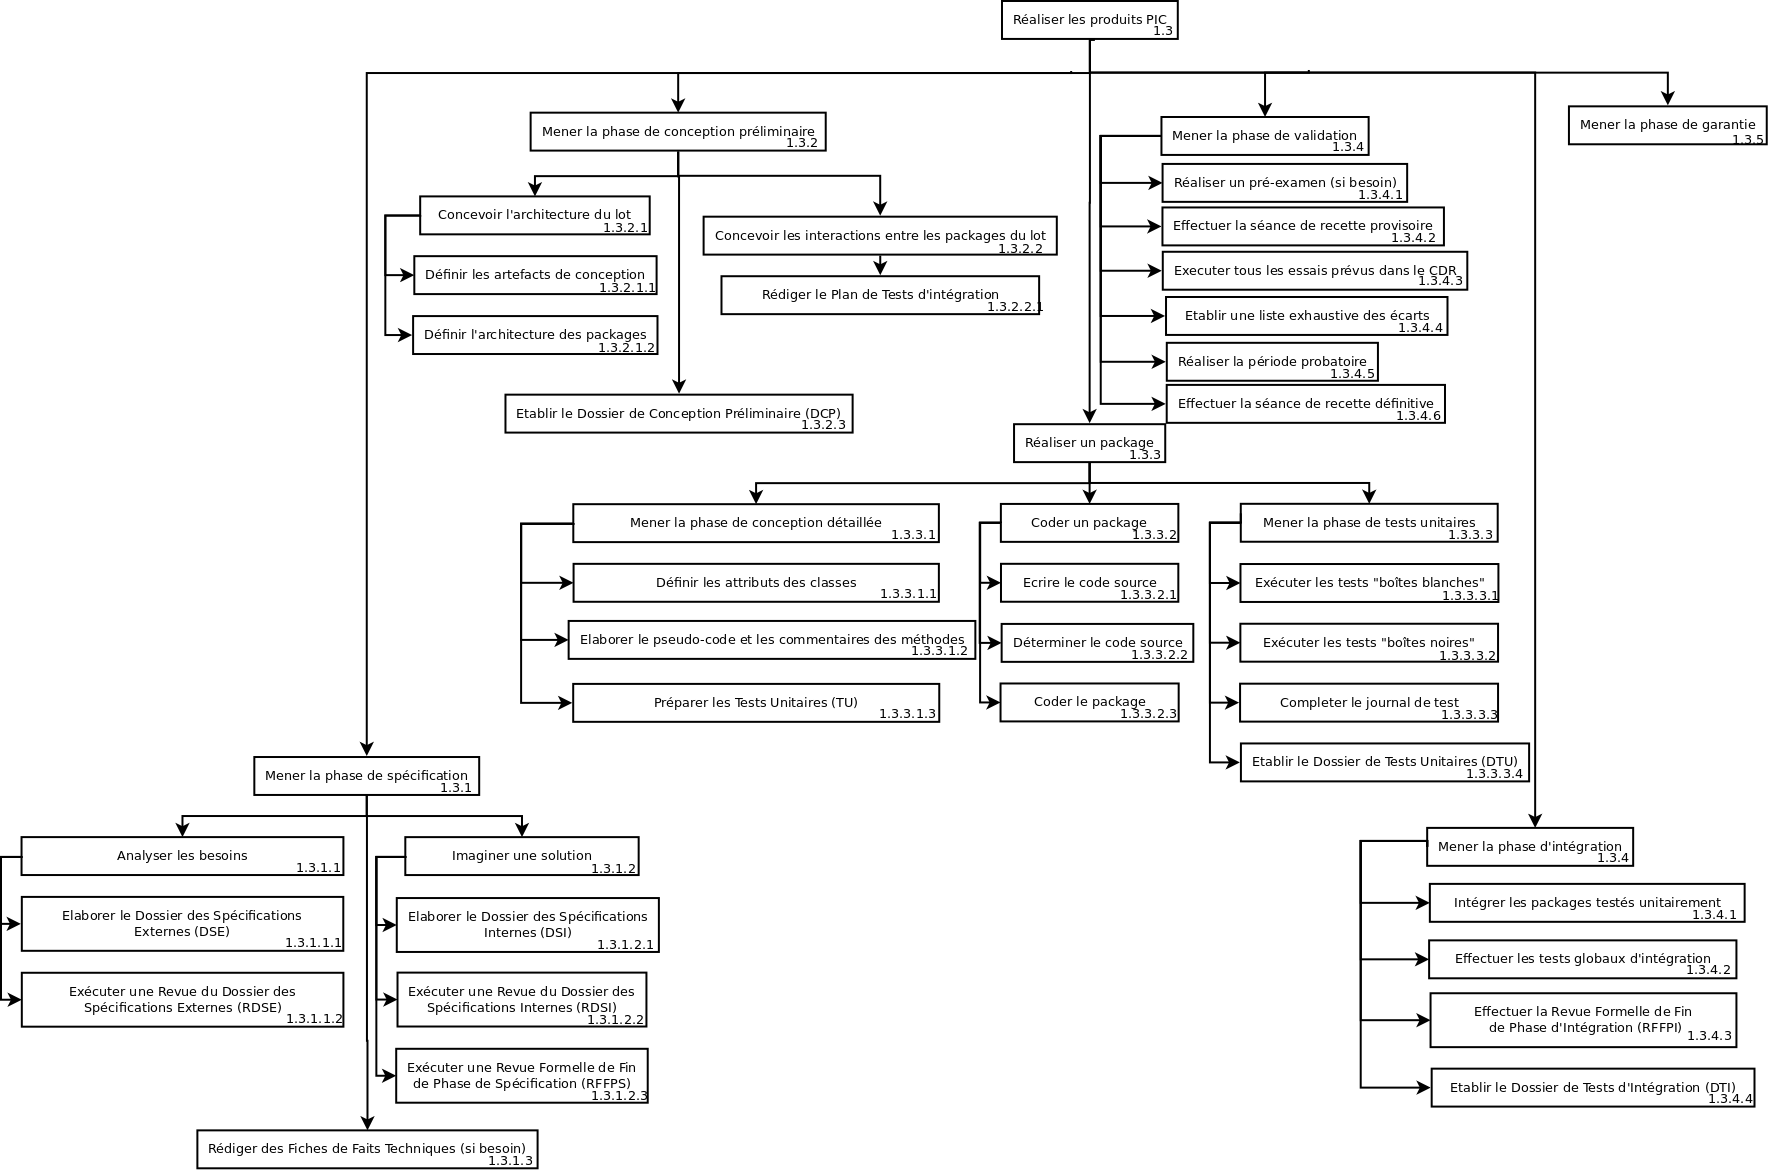
\includegraphics[width=24cm,angle=-90]{images/RealiserProduits.pdf}
 \caption{\WBSCourt{}~: Réaliser les produits}
\label{WBS5}
\end{figure}


\newpage
\begin{landscape}
\subsection{Références aux procédures}
		\begin{longtable}{|p{3.0cm}|p{14.5cm}|p{5cm}|}
		% En-tête du tableau
		\hline
		\rowcolor[gray]{0.65}\textbf{N° WBS} & \textbf{Intitulé du processus / de l'activité / de la tâche} & \textbf{Procédure en référence}\\
		\hline
		\endhead % (répétée, sinon \endfirsthead)

		\ligneMaj{1.3}{Réaliser les produits}{Chapitre 6 - \DGQDEUXCourt{}}

		\ligneSup{1.3.1}{Mener la phase de spécification}{Partie 6.2 - \DGQDEUXCourt{}}
		\ligneMed{1.3.1.1}{Analyser les besoins}{}
		\ligneSub{1.3.1.1.1}{Elaborer le Dossier des Spécifications Externes (DSE)}{Partie 6.2.1 - \DGQDEUXCourt{}}
		\ligneSub{1.3.1.1.2}{Exécuter une Revue du Dossier des Spécifications Externes (RDSE)}{Partie 6.2.2 - \DGQDEUXCourt{}}
		\ligneMed{1.3.1.2}{Imaginer une solution}{}
		\ligneSub{1.3.1.2.1}{Elaborer le Dossier des Spécifications Internes (DSI)}{Partie 6.2.1 - \DGQDEUXCourt{}}
		\ligneSub{1.3.1.2.2}{Exécuter une Revue du Dossier des Spécifications Internes (RDSI)}{Partie 6.2.2 - \DGQDEUXCourt{}}
		\ligneSub{1.3.1.2.3}{Exécuter une Revue Formelle de Fin de Phase de Spécification (RFFPS)}{Partie 6.2.4 - \DGQDEUXCourt{}}
		\ligneMed{1.3.1.3}{Rédiger des Fiches de Faits Techniques (si besoin)}{Partie 6.2.3 - \DGQDEUXCourt{}}

		\ligneSup{1.3.2}{Mener la phase de conception préliminaire}{Partie 6.3 - \DGQDEUXCourt{}}
		\ligneMed{1.3.2.1}{Concevoir l'architecture du lot}{}
		\ligneSub{1.3.2.1.1}{Définir les artefacts de conception}{Partie 6.3.1 - \DGQDEUXCourt{}}
		\ligneSub{1.3.2.1.2}{Définir l'architecture des packages}{Partie 6.3.3 - \DGQDEUXCourt{}}
		\ligneMed{1.3.2.2}{Concevoir les interactions entre les packages du lot}{}
		\ligneSub{1.3.2.2.1}{Rédiger le Plan de Tests d'intégration}{Partie 6.3.5 - \DGQDEUXCourt{}}
		\ligneSub{1.3.2.3}{Établir le Dossier de Conception Préliminaire (DCP)}{Partie 6.3.4 - \DGQDEUXCourt{}}

		\ligneSup{1.3.3}{Réaliser un package}{Partie 6.4 - \DGQDEUXCourt{}}
		\ligneMed{1.3.3.1}{Mener la phase de conception détaillée}{Partie 6.4.1 - \DGQDEUXCourt{}}
		\ligneSub{1.3.3.1.1}{Définir les attributs des classes}{Partie 6.4.1 - \DGQDEUXCourt{}}
		\ligneSub{1.3.3.1.2}{Élaborer le pseudo-code et les commentaires des méthodes}{Partie 6.4.1 - \DGQDEUXCourt{}}
		\ligneSub{1.3.3.3.3}{Préparer les Tests Unitaires (TU)}{Partie 6.4.1 - \DGQDEUXCourt{}}
		\ligneMed{1.3.3.2}{Coder un package}{Partie 6.4.2 - \DGQDEUXCourt{}}
		\ligneSub{1.3.3.2.1}{Écrire le code source}{Partie 6.4.2 - \DGQDEUXCourt{}}
		\ligneSub{1.3.3.2.2}{Déterminer le code source}{Partie 6.4.2 - \DGQDEUXCourt{}}
		\ligneSub{1.3.3.2.3}{Coder le package}{Partie 6.4.2 - \DGQDEUXCourt{}}
		\ligneMed{1.3.3.3}{Mener la phase de tests unitaires}{Partie 6.4.3 - \DGQDEUXCourt{}}
		\ligneSub{1.3.3.3.1}{Exécuter les tests "boîtes blanches"}{Partie 6.4.3 - \DGQDEUXCourt{}}
		\ligneSub{1.3.3.3.2}{Exécuter les tests "boîtes noires"}{Partie 6.4.3 - \DGQDEUXCourt{}}
		\ligneSub{1.3.3.3.3}{Compléter le journal de test}{Partie 6.4.3 - \DGQDEUXCourt{}}
		\ligneSub{1.3.3.3.4}{Établir le Dossier de Tests Unitaires (DTU)}{Partie 6.4.3 - \DGQDEUXCourt{}}

		\ligneSup{1.3.4}{Mener la phase d'intégration}{Partie 6.5 - \DGQDEUXCourt{}}
		\ligneMed{1.3.4.1}{Intégrer les packages testés unitairement}{Partie 6.5 - \DGQDEUXCourt{}}
		\ligneMed{1.3.4.2}{Effectuer les tests globaux d'intégration}{Partie 6.5 - \DGQDEUXCourt{}}
		\ligneMed{1.3.4.3}{Effectuer la Revue Formelle de Fin de Phase d’Intégration (RFFPI)}{Partie 6.5 - \DGQDEUXCourt{}}
		\ligneMed{1.3.4.4}{Établir le Dossier de Tests d’Intégration (DTI)}{Partie 6.5 - \DGQDEUXCourt{}}

		\ligneSup{1.3.4}{Mener la phase de validation}{Partie 6.6 - \DGQDEUXCourt{}}
		\ligneMed{1.3.4.1}{Réaliser un pré-examen}{Partie 6.6.1 - \DGQDEUXCourt{}}
		\ligneMed{1.3.4.2}{Réaliser la période probatoire}{Partie 6.6.1 - \DGQDEUXCourt{}}
		\ligneMed{1.3.4.3}{Effectuer la séance de recette provisoire}{Partie 6.6.1 - \DGQDEUXCourt{}}
		\ligneMed{1.3.4.4}{Exécuter tous les essais prévus dans le CDR}{Partie 6.6.1 - \DGQDEUXCourt{}}
		\ligneMed{1.3.4.5}{Établir une lise exhaustive des écarts}{Partie 6.6.1 - \DGQDEUXCourt{}}
		\ligneMed{1.3.4.6}{Effectuer la séance de recette définitive}{Partie 6.6.1 - \DGQDEUXCourt{}}

		\ligneSup{1.3.5}{Mener la phase de garantie}{Partie 6.7 - \DGQDEUXCourt{}}
		\end{longtable}
\end{landscape}